\documentclass[a4paper,12pt]{article} 

%%% Работа с русским языком
\usepackage{cmap}                           % поиск в PDF
\usepackage{mathtext} 			 	       % русские буквы в формулах
\usepackage[T2A]{fontenc}               % кодировка
\usepackage[utf8]{inputenc}              % кодировка исходного текста
\usepackage[english,russian]{babel}  % локализация и переносы
\usepackage{wrapfig}
\usepackage{gensymb}
\usepackage{textcomp}
\usepackage{multirow}
\usepackage{amsmath,amsfonts,amssymb,amsthm,mathtools} % AMS
\usepackage{euscript}	 % Шрифт Евклид
\usepackage{mathrsfs} % Красивый матшрифт
\usepackage{graphicx}%Вставка картинок правильная
\usepackage{float}%"Плавающие" картинки
\usepackage{wrapfig}%Обтекание фигур (таблиц, картинок и прочего)
\title{Лабораторная работа 2.1.5 

Исследование термических эффектов при упругих деформациях}
\author{Кагарманов Радмир Б01-106}
\date{12 апреля 2022 г.}


\begin{document}

\maketitle
\newpage
\paragraph{Цель работы:}экспериментально получить закон упругой деформации резины при постоянной температуре в зависимости от растягивающей силы; измерить нагрев резины
при адиабатическом растяжении и определить её теплоёмкость.
\paragraph{В работе используется:}образец резины (тонкая полоса), закреплённый в теплоизолированном кожухе; набор грузов; термопара; цифровой осциллограф.
\paragraph{Теория\\}
Вместо того, чтобы исследовать поглощение или выделение тепла при изотермическом процессе, можно изучать изменение температуры теплоизолированного тела. Если процесс происходит быстро, то тело можно не изолировать, поскольку процессы теплообмена идут медленно. В этом случае речь идёт об изоэнтропийном расстяжении образца. Поэтому в нашем случае связь между удлинением образца и изменением его температуры может быть выражена следующей формулой
\begin{equation} \label{eq:dT}
	dT = \frac{T}{C_l}\biggr(\frac{\partial f}{\partial T}\biggl)_l dl
\end{equation}
где $C_l$ - теплоемкость образца при постоянной длине. При больших изменениях длины образца выражение~(\ref{eq:dT}) следует проинтегрировать. Изменения температуры обычной невелики, поэтому можно заменить $T$ на $T_0$:
\begin{equation} \label{eq:S_dT}
    T - T_0 = \frac{T_0}{C_l} \int\limits_{l_0}^l \biggr(\frac{\partial f}{\partial T}\biggl)_l dl
\end{equation}
Формула~(\ref{eq:S_dT}) является окончательной и может быть применена для расчетов, если известна зависимость $f$ от $l$ и $T$. Эта зависимость не может быть поулчена теоретически и берется из опыта.
У каучуков и резины модуль Юнга зависит как от удлинения, так и от температуры. Связь между $f$, $l$ и $T$ может быть описана эмпирической формулой
\begin{equation} \label{eq:f=f(l,T)}				
    f =\frac{E(T)\sigma_0}{3}\biggr[\lambda - \frac{1 + 3\alpha (T - T_0)}{\lambda^2}\biggl]
\end{equation}
Здесь $\lambda = l / l_0$, а $\sigma_0$ - начальное поперечное сечение образца. Модуль Юнга у резины пропорционален T:
\begin{equation} \label{eq:E=E(T)}
    E = \varkappa T
\end{equation}
Для вычисления термического эффекта при расстяжении резинового образца подставим (\ref{eq:f=f(l,T)}) и (\ref{eq:E=E(T)}) в (\ref{eq:S_dT}). Интегрирование даёт
\begin{equation} \label{eq:DT}
    \Delta T = T - T_0 = \frac{E \sigma_0 l_0}{6C_l} (\lambda - 1) \biggr[\lambda + 1 - \frac{2}{\lambda} (1 + 3\alpha T_0) \biggl]
\end{equation}	
\paragraph{Экспериментальная установка\\}
Схема установки приведена на рис. 1. Исследуемый образец резины 1 расположен внутри кожуха из оргстекла 2 и закреплен по торцам в двух зажимах 3, 11. Верхний зажим неподвижен, а нижний может перемещаться вдоль двух вертикальных направляющих 4. Положение нижнего зажима определяется с помощью линейки 10, размещенной позади него. К подвижному зажиму 3 подвешена легкая платформа 5, расположенная снаружи кожуха. Резина растягивается грузом Р, помещаемым на платформу. Растяжение образца может быть ограничено положением упора 7, фиксируемого винтами 6, 9 на стойках 8.	\begin{figure}[h]
	\center{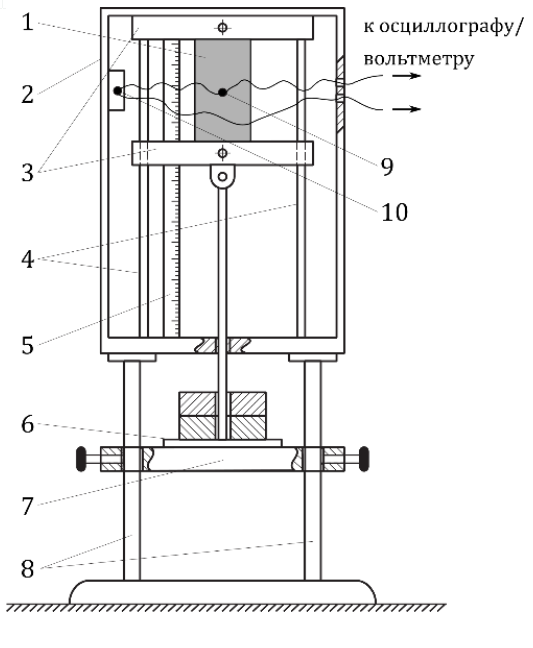
\includegraphics[width=0.5\linewidth]{Установка1.png}}
	\caption{Схема установки для исследования термических эффектов при упругой деформации резиновой пленки.}
	\label{ris:ustanovka}
\end{figure}
\paragraph{Ход работы и обработка результатов\\}
\subparagraph{1.} Характеристики установки:\\
Масса платформы: $152,0\pm 0,5 г$\\
Длина куска резины: $l_0=10,7\pm 0,1 см$\\
Ширина: $d_0 = 12,0\pm 0,5 мм$\\
Толщина: $h_0 = 1,80\pm 0,05 мм$\\
Плотность: $\rho = 1,2 \frac{г}{см^3}$\\
Чувствительность установки: $39\cdot 5000 \frac{мкВ}{\degree C}$
\subparagraph{2.}Исследуем растяжение резины, сняв несколько экспериментальных точек при разных $f$. Процесс будет изотермическим.
\begin{table}[H]
    \center
	\caption{Результаты измерений и вычислений.}
	\label{table:results_1}
	\begin{tabular}{|c|c|c|c|c|}
\hline
$m$, кг & $l$, мм & $\lambda$ & $f$, Н & $\lambda - 1/ \lambda^2$\\  \hline
0,152   & 107     & 1      & 1,49 & 0    \\ \hline
 0,317  & 113     & 1,06      &   3,107 & 0,16 \\ \hline
0,330   & 115     & 1,08      & 3,24   & 0,21                    \\ \hline
0,382   & 117     & 1,09      & 3,75   & 0,26                \\ \hline
0,405   & 119     & 1,11      & 3,97   & 0,30       \\ \hline
0,495   & 124     & 1,16      & 4,85   & 0,41       \\ \hline
0,547   & 128     & 1,20      & 5,36   & 0,50        \\ \hline
0,505 & 126 & 1,18 & 4,95 & 0,56 \\ \hline
0,557 & 129 & 1,21 & 5,46 & 0,52 \\ \hline
0,369 & 116 & 1,08 & 3,62 & 0,23 \\ \hline
0,353 & 116 & 1,08 & 3,46 & 0,23 \\ \hline
0,626 & 133 & 1,24 & 6,14 & 0,6 \\ \hline
0,681 & 138 & 1,29 & 6,68 & 0,69 \\ \hline
0,734 & 143 & 1,34 & 7,19 & 0,78 \\ \hline
0,847 & 154 & 1,44 & 8,30 & 0,96 \\ \hline
0,808 & 151 & 1,41 & 7,91 & 0,91 \\ \hline
    \end{tabular}
\end{table}
\begin{figure}[h]
	\center{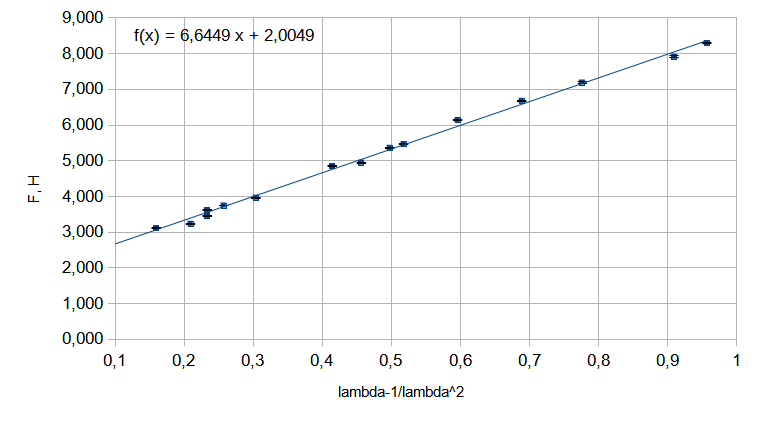
\includegraphics[width=0.7\linewidth]{F(lambda).png}}
	\caption{График зависимости $f$ от $\lambda - \frac{1}{\lambda^2}$}
	\label{ris:ustanovka}
\end{figure}
По формуле $k = \frac{Es_0}{3}$ найдём модуль Юнга. Погрешность посчитаем по формуле:
\begin{center}
    $\sigma E = E\sqrt{(\frac{\sigma h}{h})^2 + (\frac{\sigma d}{d})^2 + (\frac{\sigma k}{k})^2}$ \\
    $E = (0,92 \pm 0,09)МПа$
\end{center}
Значение модуля Юнга для различных сортов резины бывает 1-10 МПа. Полученное значение сходится по порядку величины, но точно оценить нельзя, так как мы не знаем сорт резины.
\subparagraph{3.}Построим график зависимости $A(\Delta T)$. В таблице 2 измерения изменения температуры с помощью осциоллографа.
\begin{table}[h]
    \centering
    \begin{tabular}{|c|c|c|}
    \hline
        $\Delta T, K$ & $\lambda$ & $A, Дж$ \\ \hline
        0,068 & 1,17 & 0,027\\ \hline
        0,128 & 1,25 & 0,059\\ \hline
        0,209 & 1,34 & 0,100\\ \hline
        0,250 & 1,38 & 0,128\\ \hline
        0,294 & 1,43 & 0,158\\ \hline
        0,350 & 1,49 & 0,197\\ \hline
        0,414 & 1,55 & 0,247\\ \hline
        0,509 & 1,64 & 0,319\\ \hline
    \end{tabular}
    \caption{Caption}
    \label{tab:my_label}
\end{table}
\begin{figure}[h]
	\center{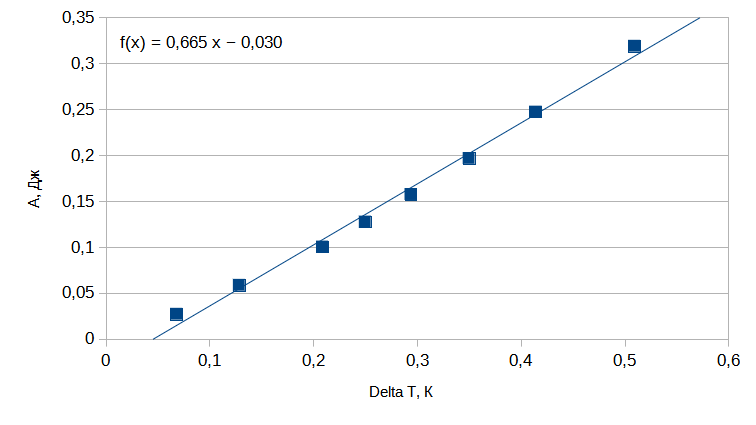
\includegraphics[width=0.7\linewidth]{AT.png}}
	\caption{График зависимости $A$ от $\Delta T$}
	\label{ris:ustanovka}
\end{figure}\\
$A=C_l\cdot \Delta T\Rightarrow C_l = 0,665\pm 0,086 \frac{Дж}{К} = 0,159\pm 0,021\frac{кал}{К}$\\
На установке было написано, что теплоёмкость резины лежит в интервале $0,27\div0,5 \frac{кал}{град.}$. Полученное значение не попало в этот интервал, но оно сходится с ним по порядку величины.
\subparagraph{4.}Найдём удельную теплоёмкость.
$c_l = \frac{C_l}{l_0 h_0 d_0 \rho}=239,8\pm 31,2 \frac{Дж}{кг\cdot К}$\newpage
\subparagraph{5.}Из формулы коэффициента теплового расширения $\alpha = \frac{1}{l}(\frac{\partial l}{\partial T})_f$ видно, что он измеряется в $[\text{K}^{-1}]$. \\
Найдём $\alpha$ из формулы $(\frac{\partial T}{\partial l})_s = -\frac{\alpha l(\frac{\partial f}{\partial l})_s T}{C_l}$.
\begin{center}
    $\alpha = -3,7\cdot 10^{-3} K^{-1}$\\
\end{center}
\begin{figure}[h]
	\center{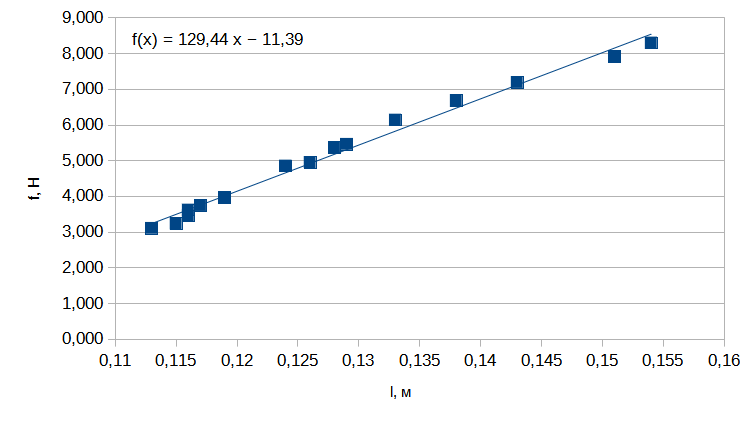
\includegraphics[width=0.7\linewidth]{fl.png}}
	\caption{График зависимости $f$ от $l$}
	\label{ris:ustanovka}
\end{figure}
\begin{figure}[h]
	\center{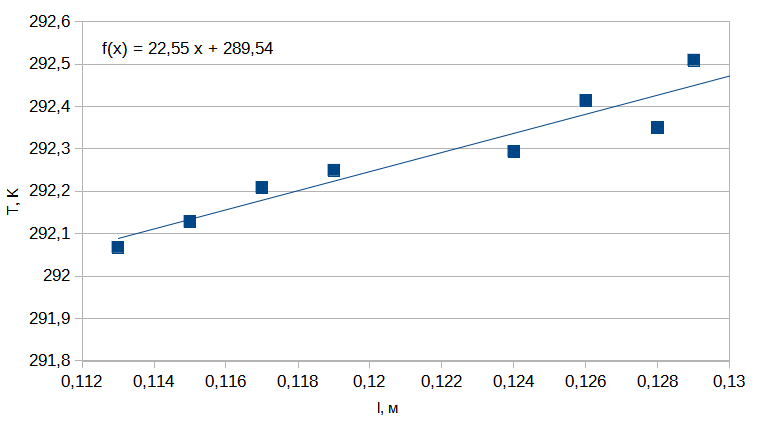
\includegraphics[width=0.7\linewidth]{Tl.png}}
	\caption{График зависимости $T$ от $l$}
	\label{ris:ustanovka}
\end{figure}\\
\newpage
\paragraph{Вывод:}в ходе лабораторной работы мы проверили закон Гука, посчитали модуль Юнга, изотермическое и адиабатическое растяжение резины, из которого вычислили теплоёмкость куска резины.
\end{document}
